\documentclass[a4paper,fleqn,12pt]{article}
\usepackage[utf8]{inputenc}
\usepackage{amsmath}
\usepackage{amssymb}
\usepackage{booktabs}
\usepackage{fancyhdr}
\usepackage{amsthm}
\usepackage{graphicx}
\usepackage{pdfpages}

\begin{document}
\begin{titlepage}
	\setlength{\parindent}{0pt}
	\large
\centering
Techincal University - Sofia \par
Faculty of Applied Mathematics and Informatics \par
\vspace{2cm}

{\huge Project 1 - Topics of Algebra\par}

\vspace{2cm}

\vspace{1cm}
{\LARGE\scshape  Solution for version 4 \par}



\vfill

\begin{minipage}[t]{.5\linewidth}
	Student: \\
	Kristian Krachmarov \\
	791324005
\end{minipage}%
\begin{minipage}[t]{.5\linewidth}
	\raggedleft
	Examiner:\\
	Prof Mirko Tarulli
\end{minipage}

\vspace{2cm}
\raggedright

\end{titlepage}
\pagenumbering{gobble}
\tableofcontents
\newpage
%\fontsize{14pt}{16pt}\selectfont
\pagenumbering{arabic}
\newpage

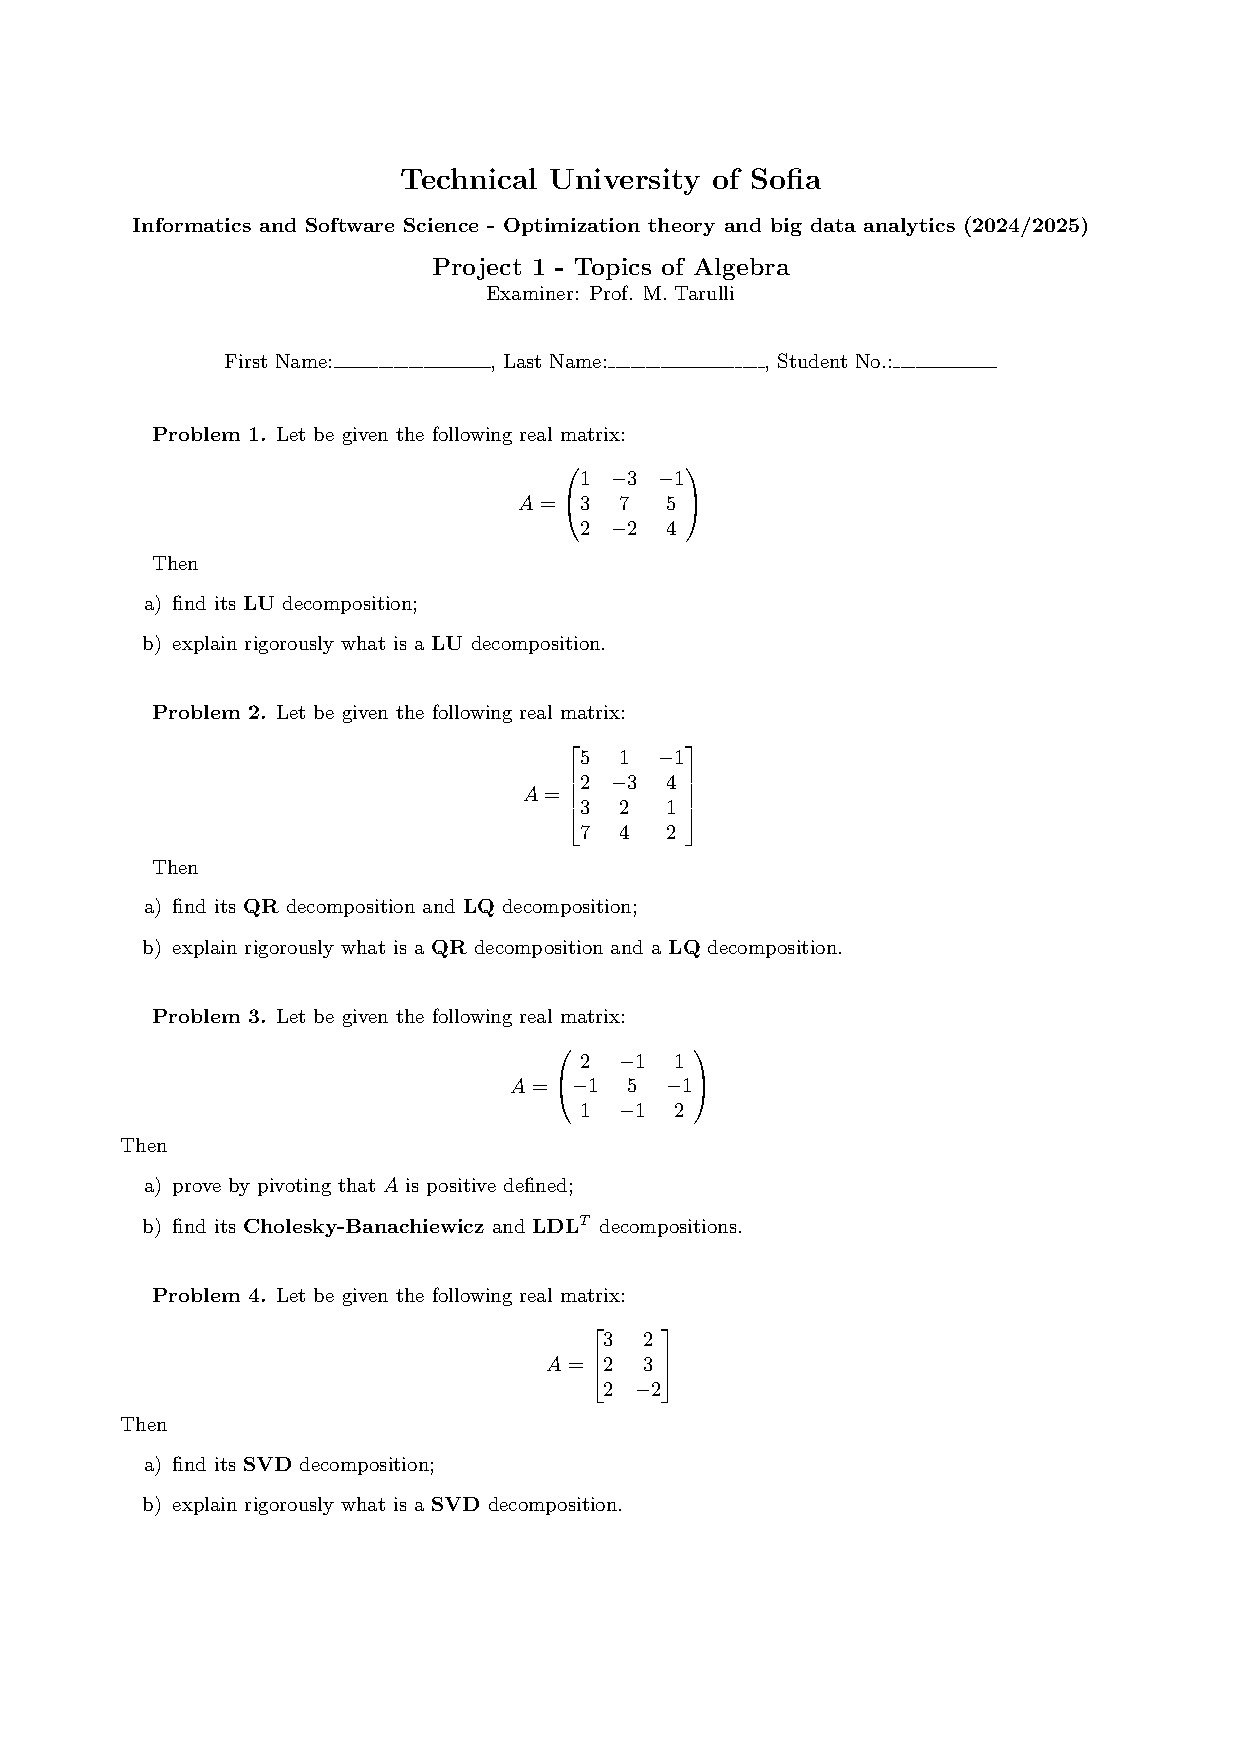
\includepdf[pages=-]{Project1-Version4-2425.pdf}
\newpage

\section{Problem 1}
\subsection{Solution for 1a}
\subsection{Solution for 1b}

\newpage

\section{Problem 2}
\subsection{Solution for 2a}
\subsection{Solution for 2b}
\newpage

\section{Problem 3}
\subsection{Solution for 3a}
\subsection{Solution for 3b}
\newpage

\section{Problem 4}
\subsection{Solution for 4a}
\subsection{Solution for 4b}


















































\end{document}